\documentclass[conference]{IEEEtran}
\usepackage{amsmath,amssymb,amsfonts}
% \IEEEoverridecommandlockouts
%
%my custom settings
\usepackage{fontspec}
\usepackage{unicode-math}
\setmainfont{Times New Roman}
\setmathfont[Scale=1]{Asana Math}
\usepackage{algorithmic}
\usepackage{graphicx}
\graphicspath{{./images/}}
\usepackage{textcomp}
\usepackage{xcolor}

\usepackage{tabularx}
%mathcha includes
\usepackage{physics}
\usepackage{tikz}
\usepackage{mathdots}
\usepackage{cancel}
\usepackage{color}
\usepackage{siunitx}
\usepackage{array}
\usepackage{multirow}
\usepackage{gensymb}
\usepackage{tabularx}
\usepackage{booktabs}
\usetikzlibrary{fadings}
\usetikzlibrary{patterns}
\usetikzlibrary{shadows.blur}
\usetikzlibrary{shapes}


\def\BibTeX{{\rm B\kern-.05em{\sc i\kern-.025em b}\kern-.08em
    T\kern-.1667em\lower.7ex\hbox{E}\kern-.125emX}}
\begin{document}

\title{EE 4202 Laboratory in Circuits}

\author{\IEEEauthorblockN{Stephen Campbell}}
\maketitle

\begin{abstract}
    %TODO 
    In this lab the speed of light was measured and familiarity with scalar RF power measurements was gained.
\end{abstract}

\section{Introduction}
    %TODO 
This document is a model and instructions for \LaTeX.
Please observe the conference page limits. 

\section{Measuring the speed of light}

\subsection{Procedure}

To measure the speed of light using a microwave, the rotating plate was removed
from the microwave. Sliced cheese was the placed onto a paper plate inside of
the microwave. After 15 seconds in the microwave the cheese platter was
examined. There were regions of soft, melted cheese and hard, cold cheese.
Because the microwave forms standing waves during operation, it is implied that
the hot spots correspond to the standing waves antinodes. The distance between
adjacent antinodes corresponds to have wavelengths of the standing wave. Using
this to determine the wavelength.

\begin{table}[htbp]
    \begin{center}
        \begin{tabular}{|c|c|}
            \hline
            \textbf{Measurement Type}         & \textbf{Value} \\ \hline
            Frequency of microwave operation: & 2.45 GHz       \\ \hline
            Distance between hotspots         & 5.75 cm        \\ \hline
        \end{tabular}
    \end{center}
\end{table}

\begin{align*}
\frac{\lambda }{2} & =5.75\times 10^{-2}\text{m}\\
\lambda  & =11.5\times 10^{-2}\text{m}\\
f & =2.45\times 10^{9}\text{Hz}\\
 & \\
c_{\text{measured}} & =\lambda f\\
c_{\text{measured}} & =\left( 11.5\times 10^{-2}\right)\left( 2.45\times 10^{9}\right)\\
c_{\text{measured}} & =2.8175\times 10^{8} \\
\end{align*}
\begin{align*}
\%\ \text{error} & =\frac{|c-c_{\text{measured}}{} |}{c}\\
\%\ \text{error} & =\frac{|2.99\times 10^{8} -2.8175\times 10^{8} |}{2.99\times 10^{8}} \cdot 100\%\\
\%\ \text{error} & =0.05\ \cdot 100\%\\
\%\ \text{error} & =5\%
\end{align*}


\subsection{Analysis}

The accuracy of the speed of light measurement was dependent on several factors.
The factors likely caused the drift between the measured speed of light and the
theoretical speed of light. These factors include but are not limited to:
\begin{itemize}
    \item Tolerance of the generated frequency of the microwave 
    \item Measurement error using the ruler
    \item Operator error related to the ambiguity of the exact location of the antinodes
\end{itemize}
With these in mind, the percent error of 5\% is entirely reasonable. Some
problems include the ambiguity with the exact location of the antinodes as it
seemed as if the antinodes occurred at the seams of the cheese slices. A
solution to fix this problem would be to procure a larger cheese sheet and to
leave the microwave on for longer. With these 2 modifications the ambiguity of
the antinode location would be minimized. Another problem is the limited sample
size. This subjects the measured value to random errors. By collecting more
samples, one could gain more confidence in the measurements.

\subsection{Question to Consider}

\textbf{From what you learned in lab today why do microwave oven manufacturers
almost always include a rotating platform?}

The rotating platform reduces the uneven heating that the microwave produces.
From the food’s perspective, the nodes/antinodes are constantly changing
positions so the food cooks more evenly than it would be otherwise.    

\section{Scalar Power Measurements}

\subsection{Attenuators}
The measured power of the signal generator's 2GHz 0dBm signal was -0.12 dBm. For
a 2 GHz frequency, several measurements were made.
\begin{table*}[htbp]
\begin{tabular}{|l p{3em}|l p{3em}|l p{3em}|l p{3em}|l p{3em}|l p{3em}|}
\hline
\textbf{Medium}     & \textbf{Absolute Power (dBm)} & \textbf{Absolute Power (mW)} & \textbf{Insertion Loss (dB) at 2GHz} & \textbf{Insertion Loss Difference Absolute (dB)} & \textbf{Insertion Loss Difference Percentage} \\ \hline
RF Cable            & -0.12                         & 0.972747                     & -0.12                                & N/A                                              & N/A                                           \\ \hline
3dB SMA attenuator  & -3.8                          & 0.416869                     & -3.8                                 & -0.8                                             & 26.667                                        \\ \hline
10dB SMA attenuator & -10.28                        & 0.0937562                    & -10.28                               & -0.28                                            & 2.8                                           \\ \hline
20dB SMA attenuator & -20.17                        & 0.00961612                   & -20.17                               & -0.17                                            & 0.85                                          \\ \hline
\end{tabular}
\end{table*}
\subsection{Filter}

\begin{table}[htbp]
\begin{tabular}{|l|l|}
\hline
\textbf{Frequency (GHz)} & \textbf{Absolute Power (dBm)} \\ \hline
1                        & -36.00                        \\ \hline
1.25                     & -34.42                        \\ \hline
1.5                      & -40                           \\ \hline
1.75                     & -28                           \\ \hline
2                        & -9.32                         \\ \hline
2.25                     & -1.86                         \\ \hline
2.5                      & -2.07                         \\ \hline
2.75                     & -6.94                         \\ \hline
3                        & -12.99                        \\ \hline
3.25                     & -12.6                         \\ \hline
3.5                      & -23.47                        \\ \hline
3.75                     & -27.10                        \\ \hline
4                        & -32.01                        \\ \hline
\end{tabular}
\end{table}

\begin{figure}[htbp]
\centerline{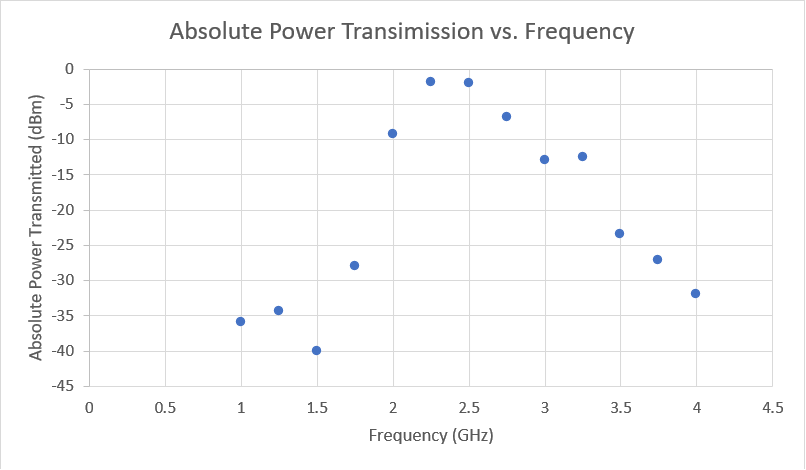
\includegraphics[width=0.4\textwidth]{filter_transmission.png}}
% \caption{}
\label{Filter Power Transmission}
\end{figure}

\section{Appendix}

\begin{figure}[htbp]
\centerline{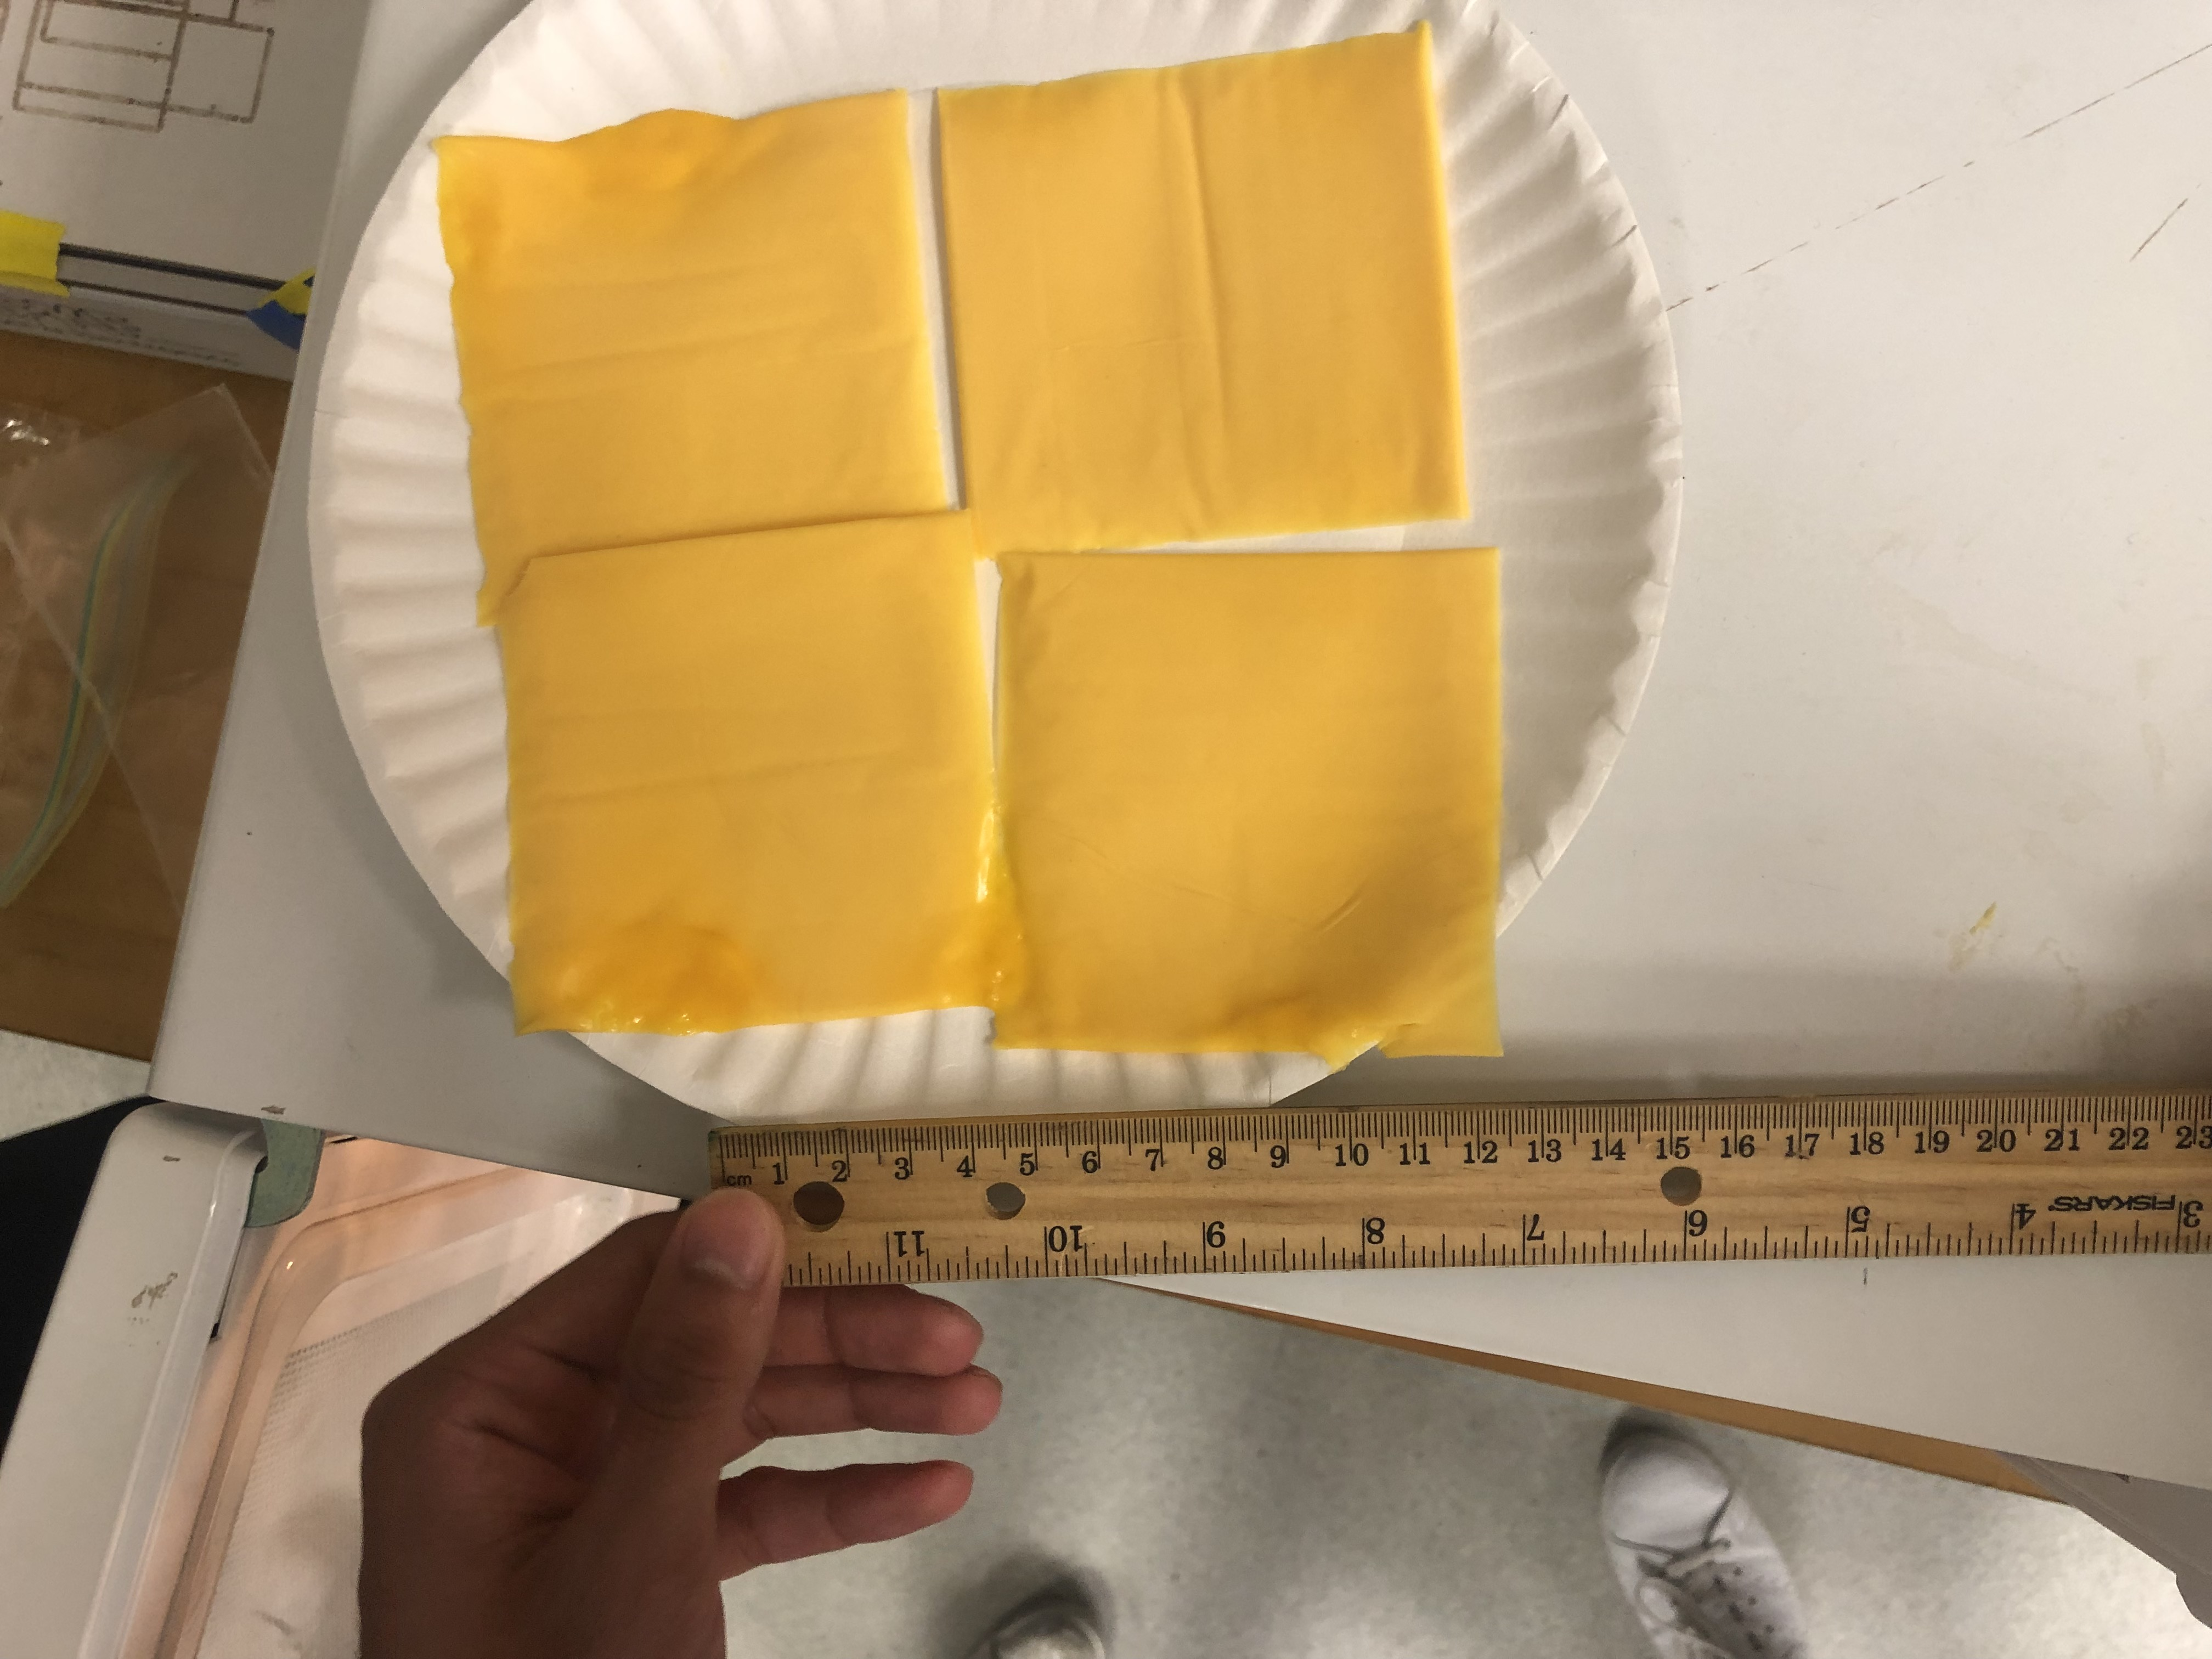
\includegraphics[width=0.3\textwidth]{cheese.jpg}}
\caption{Cheese slices that were measured to determine the speed of light}
\label{Cheese Slice Measurment Setup}
\end{figure}


% Table Example
% \begin{table}[htbp]
% \caption{Table Type Styles}
% \begin{center}
% \begin{tabular}{|c|c|c|c|}
% \hline
% \textbf{Table}&\multicolumn{3}{|c|}{\textbf{Table Column Head}} \\
% \cline{2-4} 
% \textbf{Head} & \textbf{\textit{Table column subhead}}& \textbf{\textit{Subhead}}& \textbf{\textit{Subhead}} \\
% \hline
% copy& More table copy$^{\mathrm{a}}$& &  \\
% \hline
% \multicolumn{4}{l}{$^{\mathrm{a}}$Sample of a Table footnote.}
% \end{tabular}
% \label{tab1}
% \end{center}
% \end{table}


% Figure Example 
% \begin{figure}[htbp]
% \centerline{\includegraphics{fig1.png}}
% \caption{Example of a figure caption.}
% \label{fig}
% \end{figure}

\end{document}
